\subsection{Recap: Process Models}
% waterfall, V-model, scrum, ...

\subsection{Domain Engineering}

\subsubsection{Domain Analysis}
% domain-driven requirements analysis, crucial, not always explicit
% scoping!
\begin{frame}{Scoping in Practice}
	\centering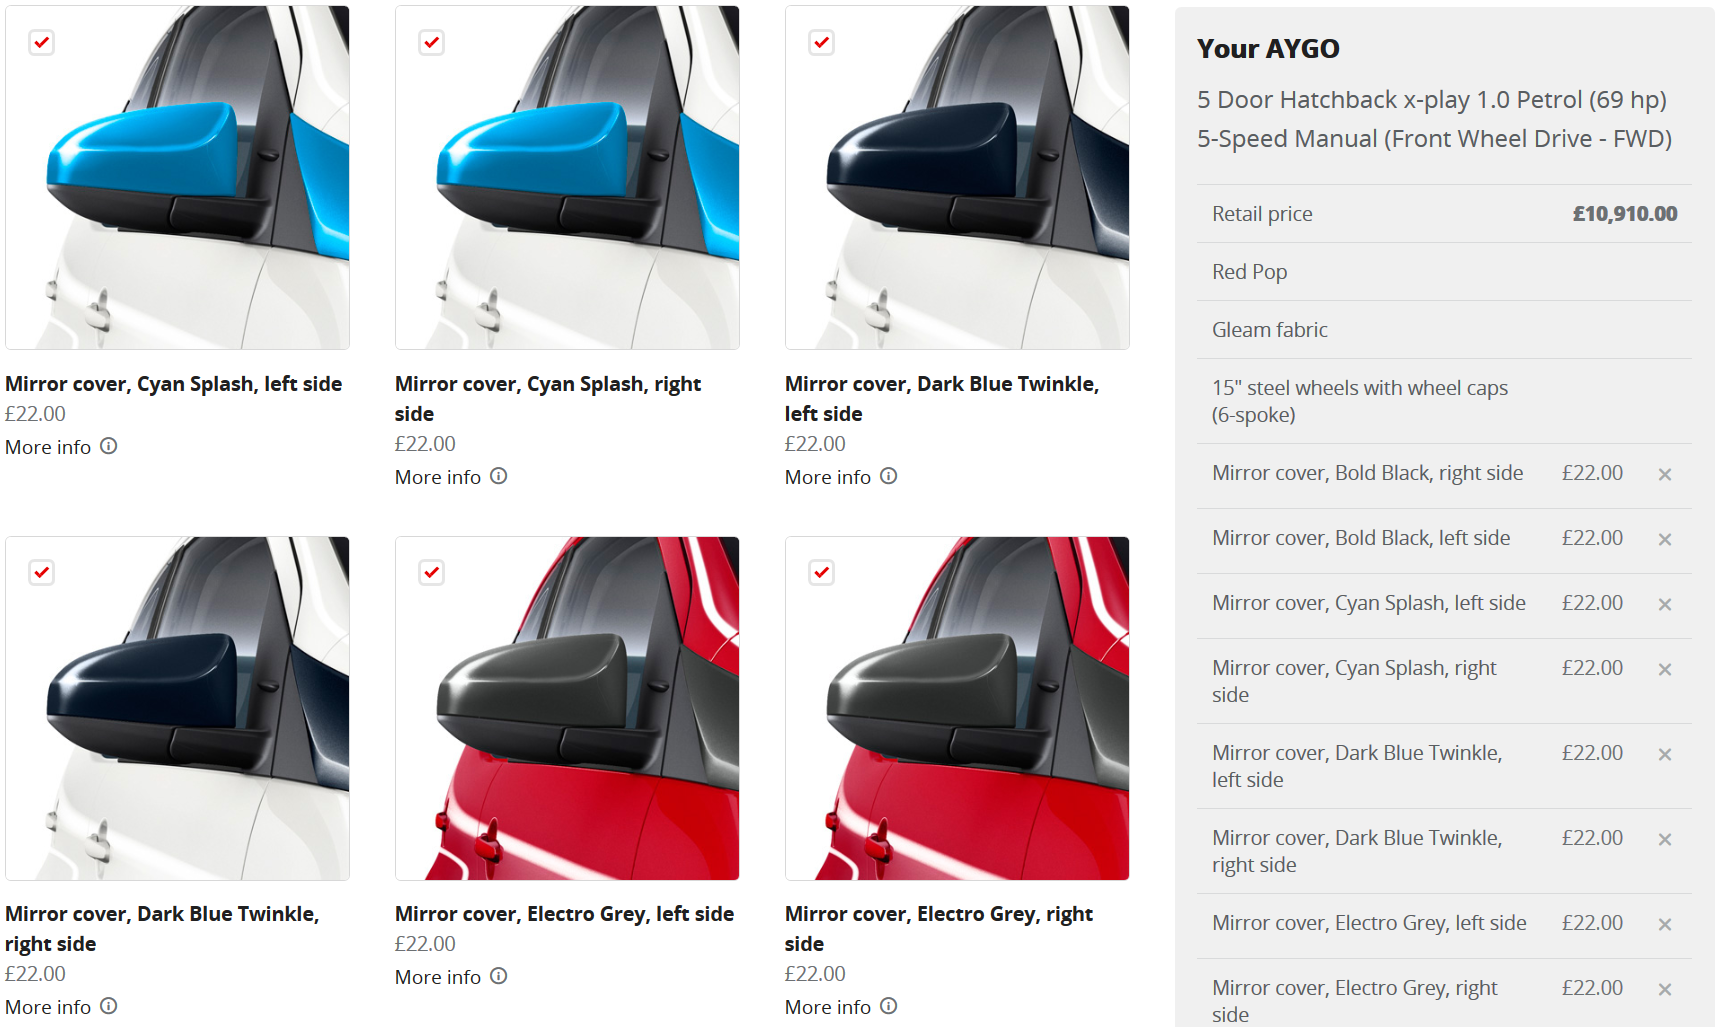
\includegraphics[width=.8\linewidth]{toyota-aygo-mirrorcovers}
\end{frame}

\subsubsection{Domain Design and Implementation}
% reusable parts indespensible, reusable architecture optional
\subsubsection{Domain Testing/Verification}
% systematic testing, sometimes skipped (e.g., if product derivation not automatic)

\subsection{Application Engineering}

\subsubsection{Product Configuration}
% application-specific requirements analysis
\subsubsection{Application Design and Implementation}
% fully automatic or semi-automatic with custom design and implementation
\subsubsection{Application Testing/Verification}
% testing of a single product, sometimes optional

\subsection{Overview on Domain and Application Engineering}
% overview picture, also to wrap-up

% lecture 8: show how linux in lecture 4+5 relates to problem space (kconfig)/mapping (kbuild)/solution space (cpp) - put this into the four-quadrant model

